\section{Quantum Machine Learning}

\begin{figure}[htb]
    \centering
    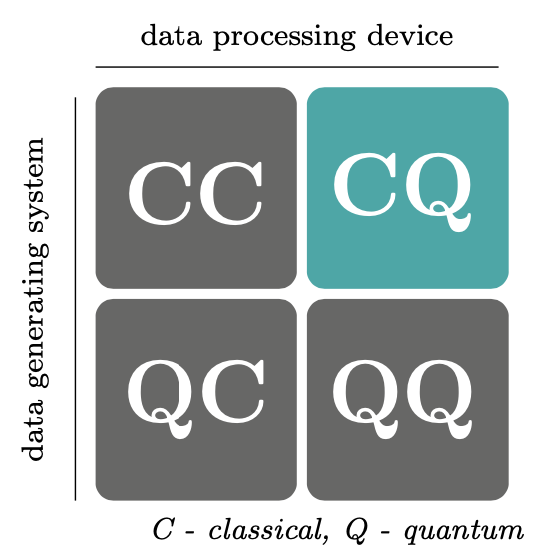
\includegraphics[keepaspectratio, scale=0.5]{introduction/4types.jpeg}
    \caption{4 types of quamtum machine learning.}
    \label{fig:4types}
\end{figure}

\par The idea of machine learning using quantum computers already existed at the dawn of quantum computers in the 1980s. The quantum model of neural networks was proposed in 1995 \cite{quest} and in 2000 \cite{assomem}. However, these studies were sporadic and did not attract enough attention to make quantum machine learning a major research topic. 

\par Quantum machine learning research has become popular just recently. Peter Wittek wrote a monograph \textit{Quantum Machine Learning— What quantum computing means to data mining} in 2014, which brought attention to quantum machine learning. Now quantum machine learning is one of the most vigorously studied fields in quantum computing research, and its research scope is wide-ranging.

\par The research of quantum machine learning can be divided into four types, which was proposed by Aimeur, Brassard and Gambs \cite{4types} (in Figure \ref{fig:4types}). These 4 types are divided by the assumptions whether the data is generated quantum (Q) or classically (C), and whether information is processed quantum (Q) or classically (C). 

\par CC means machine learning with classical data by using classical computers. CC is basically a conventional machine learning approach, but here it stands for machine learning that makes use of the knowledge of quantum computing. An example of the research of CC is \textit{tensor network} \cite{tensor1, tensor2}: tensor network is inspired by methods used to simulate quantum systems as efficiently as possible in classical computers, and now investigated for the purpose of processing high-dimensional data approximately in low-dimensional. 

\par QC means machine learning with quantum generated data by classical computations. QC is mainly aimed at simulating phenomena peculiar to quantum with classical computers. \cite{entannn,tomogra}

\par QQ means machine learning "quantum data" with the help of quantum computers. "Quantum data" is made up of quantum states generated by quantum computers, and after the generation directly used as the training dataset.

\par CQ means machine learning of classical data with the help of quantum computers. The classical data has to be encoded as a quantum state so that quantum computers are able to analyze it. 

\par This work focuses on supervised machine learning of classical data with the help of quantum computers, henceforth when we refer to quantum machine learning we mean CQ-type supervised machine learning.

\par Quantum-classical hybrid algorithms are said to be promising for quantum computing in the NISQ era when only approximate solutions can be obtained and the scale of quantum circuit executable is limited. Hybrid algorithms are widely used in quantum machine learning, and quantum devices are mainly used to produce the models, and classical computers fix those models to fit the given data.

\par There are two basic methods for quantum machine learning (sometimes used in other fields like quantum optimization, quantum eigenvalue solver, etc.), kernel method and variational method. These are quantum-classical hybrid algorithms, as mentioned earlier.